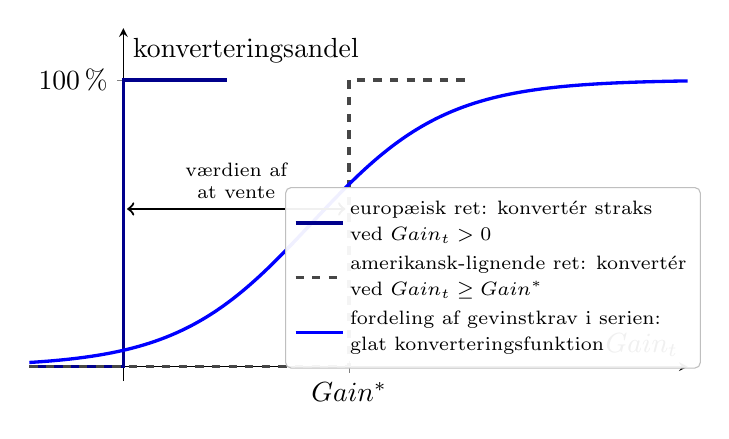
\begin{tikzpicture}
\begin{axis}[
    width=0.82\textwidth,
    height=0.50\textwidth,
    xlabel={$Gain_t$},
    ylabel={konverteringsandel},
    xmin=-0.05, xmax=0.30,
    ymin=-0.05, ymax=1.18,
    axis lines=middle,
    ytick={1},
    yticklabels={100\,\%},
    xtick={0,0.12},
    xticklabels={$0$,$Gain^{*}$},
    domain=-0.05:0.30,
    samples=150,
    clip=false,
    legend style={
    at={(1.02,0.55)},
    anchor=north east,
    font=\scriptsize,
    draw=gray!50,
    fill=white,
    fill opacity=0.94,
    text opacity=1,
    rounded corners=2pt,
    inner sep=3pt
    },
    legend cell align=left
]

% (1) Europæisk ret: konverter straks ved Gain > 0
\addplot[very thick, blue!55!black]
    coordinates {(-0.05,0) (0,0) (0,1) (0.055,1)};
\addlegendentry{
    \shortstack[l]{europæisk ret: konvertér straks\\
    ved $Gain_t>0$}
}

% (2) Amerikansk-lignende ret: gevinstkrav
\addplot[very thick, dashed, gray!55!black]
    coordinates {(-0.05,0) (0.12,0) (0.12,1) (0.185,1)};
\addlegendentry{
    \shortstack[l]{amerikansk-lignende ret: konvertér\\
    ved $Gain_t\geq Gain^{*}$}
}

% (3) Fordeling over låntagere: glat kurve
\addplot[very thick, blue]
    {1/(1+exp(-28*(x-0.10)))};
\addlegendentry{
    \shortstack[l]{fordeling af gevinstkrav i serien:\\
    glat konverteringsfunktion}
}

% Værdien af at vente
\draw[<->, thick]
    (axis cs:0.002,0.55) -- (axis cs:0.118,0.55)
    node[midway, above, font=\scriptsize, align=center]
    {værdien af\\at vente};

\end{axis}
\end{tikzpicture}
